% Graphic for TeX using PGF
% Title: /home/nevj/common/Fleece-biology/diamlen/compoundfoll/Diagram1.dia
% Creator: Dia v0.97.3
% CreationDate: Wed Oct 24 20:20:57 2018
% For: nevj
% \usepackage{tikz}
% The following commands are not supported in PSTricks at present
% We define them conditionally, so when they are implemented,
% this pgf file will use them.
%\begin{document}
%\begin{landscape}
%\label{fig:diampath}
\begin{figure}[!h]
  \centering

\ifx\du\undefined
  \newlength{\du}
\fi
\setlength{\du}{15\unitlength}
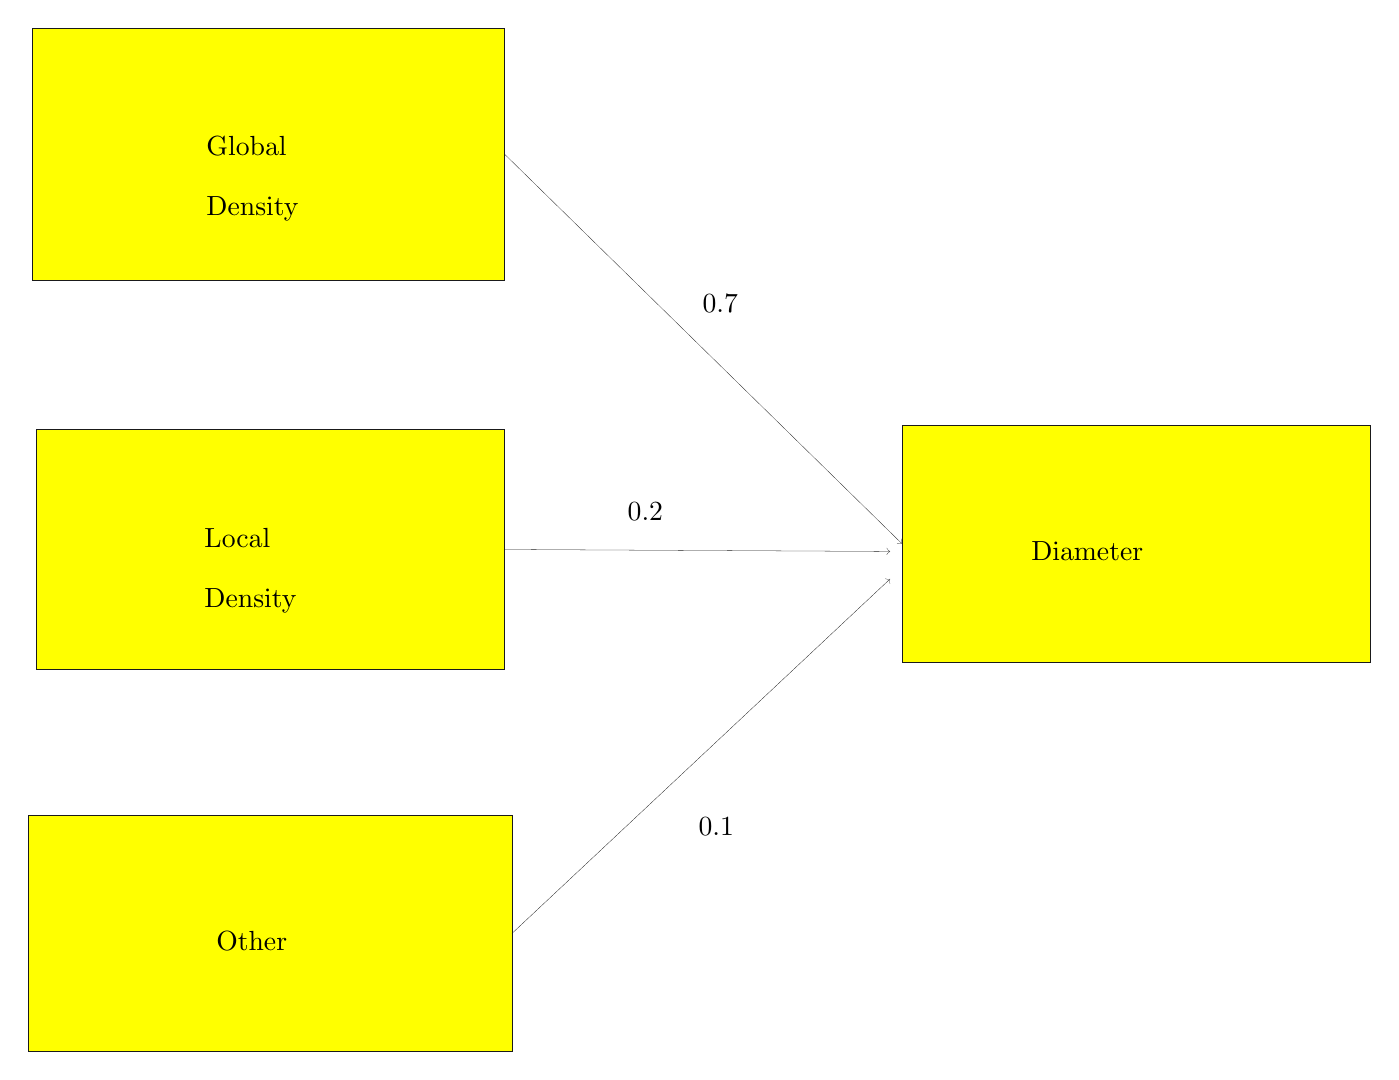
\begin{tikzpicture}
\pgftransformxscale{1.000000}
\pgftransformyscale{-1.000000}
\definecolor{dialinecolor}{rgb}{0.000000, 0.000000, 0.000000}
\pgfsetstrokecolor{dialinecolor}
\definecolor{dialinecolor}{rgb}{1.000000, 1.000000, 1.000000}
\pgfsetfillcolor{dialinecolor}
\pgfsetlinewidth{0.100000\du}
\pgfsetdash{}{0pt}
\pgfsetdash{}{0pt}
\pgfsetmiterjoin
\definecolor{dialinecolor}{rgb}{1.000000, 1.000000, 0.000000}
\pgfsetfillcolor{dialinecolor}
\fill (2.000000\du,1.950000\du)--(2.000000\du,5.150000\du)--(8.000000\du,5.150000\du)--(8.000000\du,1.950000\du)--cycle;
\definecolor{dialinecolor}{rgb}{0.101961, 0.101961, 0.101961}
\pgfsetstrokecolor{dialinecolor}
\draw (2.000000\du,1.950000\du)--(2.000000\du,5.150000\du)--(8.000000\du,5.150000\du)--(8.000000\du,1.950000\du)--cycle;
\pgfsetlinewidth{0.100000\du}
\pgfsetdash{}{0pt}
\pgfsetdash{}{0pt}
\pgfsetmiterjoin
\definecolor{dialinecolor}{rgb}{1.000000, 1.000000, 0.000000}
\pgfsetfillcolor{dialinecolor}
\fill (2.050000\du,7.050000\du)--(2.050000\du,10.100000\du)--(8.000000\du,10.100000\du)--(8.000000\du,7.050000\du)--cycle;
\definecolor{dialinecolor}{rgb}{0.101961, 0.101961, 0.101961}
\pgfsetstrokecolor{dialinecolor}
\draw (2.050000\du,7.050000\du)--(2.050000\du,10.100000\du)--(8.000000\du,10.100000\du)--(8.000000\du,7.050000\du)--cycle;
\pgfsetlinewidth{0.100000\du}
\pgfsetdash{}{0pt}
\pgfsetdash{}{0pt}
\pgfsetmiterjoin
\definecolor{dialinecolor}{rgb}{1.000000, 1.000000, 0.000000}
\pgfsetfillcolor{dialinecolor}
\fill (1.950000\du,11.950000\du)--(1.950000\du,14.950000\du)--(8.100000\du,14.950000\du)--(8.100000\du,11.950000\du)--cycle;
\definecolor{dialinecolor}{rgb}{0.101961, 0.101961, 0.101961}
\pgfsetstrokecolor{dialinecolor}
\draw (1.950000\du,11.950000\du)--(1.950000\du,14.950000\du)--(8.100000\du,14.950000\du)--(8.100000\du,11.950000\du)--cycle;
\pgfsetlinewidth{0.100000\du}
\pgfsetdash{}{0pt}
\pgfsetdash{}{0pt}
\pgfsetmiterjoin
\definecolor{dialinecolor}{rgb}{1.000000, 1.000000, 0.000000}
\pgfsetfillcolor{dialinecolor}
\fill (13.050000\du,7.000000\du)--(13.050000\du,10.000000\du)--(19.000000\du,10.000000\du)--(19.000000\du,7.000000\du)--cycle;
\definecolor{dialinecolor}{rgb}{0.101961, 0.101961, 0.101961}
\pgfsetstrokecolor{dialinecolor}
\draw (13.050000\du,7.000000\du)--(13.050000\du,10.000000\du)--(19.000000\du,10.000000\du)--(19.000000\du,7.000000\du)--cycle;
% setfont left to latex
\definecolor{dialinecolor}{rgb}{0.101961, 0.101961, 0.101961}
\pgfsetstrokecolor{dialinecolor}
\node[anchor=west] at (16.025000\du,8.500000\du){};
% setfont left to latex
\definecolor{dialinecolor}{rgb}{0.101961, 0.101961, 0.101961}
\pgfsetstrokecolor{dialinecolor}
\node[anchor=west] at (16.025000\du,8.500000\du){};
% setfont left to latex
\definecolor{dialinecolor}{rgb}{0.101961, 0.101961, 0.101961}
\pgfsetstrokecolor{dialinecolor}
\node[anchor=west] at (14.575000\du,8.600000\du){Diameter};
% setfont left to latex
\definecolor{dialinecolor}{rgb}{0.101961, 0.101961, 0.101961}
\pgfsetstrokecolor{dialinecolor}
\node[anchor=west] at (4.100000\du,3.450000\du){Global };
% setfont left to latex
\definecolor{dialinecolor}{rgb}{0.101961, 0.101961, 0.101961}
\pgfsetstrokecolor{dialinecolor}
\node[anchor=west] at (4.100000\du,4.250000\du){Density};
% setfont left to latex
\definecolor{dialinecolor}{rgb}{0.101961, 0.101961, 0.101961}
\pgfsetstrokecolor{dialinecolor}
\node[anchor=west] at (4.075000\du,8.425000\du){Local};
% setfont left to latex
\definecolor{dialinecolor}{rgb}{0.101961, 0.101961, 0.101961}
\pgfsetstrokecolor{dialinecolor}
\node[anchor=west] at (4.075000\du,9.225000\du){Density};
% setfont left to latex
\definecolor{dialinecolor}{rgb}{0.101961, 0.101961, 0.101961}
\pgfsetstrokecolor{dialinecolor}
\node[anchor=west] at (4.225000\du,13.550000\du){Other};
\pgfsetlinewidth{0.100000\du}
\pgfsetdash{}{0pt}
\pgfsetdash{}{0pt}
\pgfsetbuttcap
{
\definecolor{dialinecolor}{rgb}{0.101961, 0.101961, 0.101961}
\pgfsetfillcolor{dialinecolor}
% was here!!!
\pgfsetarrowsend{to}
\definecolor{dialinecolor}{rgb}{0.101961, 0.101961, 0.101961}
\pgfsetstrokecolor{dialinecolor}
\draw (8.000000\du,3.550000\du)--(13.050000\du,8.500000\du);
}
\pgfsetlinewidth{0.100000\du}
\pgfsetdash{}{0pt}
\pgfsetdash{}{0pt}
\pgfsetbuttcap
{
\definecolor{dialinecolor}{rgb}{0.101961, 0.101961, 0.101961}
\pgfsetfillcolor{dialinecolor}
% was here!!!
\pgfsetarrowsend{to}
\definecolor{dialinecolor}{rgb}{0.101961, 0.101961, 0.101961}
\pgfsetstrokecolor{dialinecolor}
\draw (8.000000\du,8.575000\du)--(12.900000\du,8.600000\du);
}
\pgfsetlinewidth{0.100000\du}
\pgfsetdash{}{0pt}
\pgfsetdash{}{0pt}
\pgfsetbuttcap
{
\definecolor{dialinecolor}{rgb}{0.101961, 0.101961, 0.101961}
\pgfsetfillcolor{dialinecolor}
% was here!!!
\pgfsetarrowsend{to}
\definecolor{dialinecolor}{rgb}{0.101961, 0.101961, 0.101961}
\pgfsetstrokecolor{dialinecolor}
\draw (8.100000\du,13.450000\du)--(12.900000\du,8.950000\du);
}
% setfont left to latex
\definecolor{dialinecolor}{rgb}{0.101961, 0.101961, 0.101961}
\pgfsetstrokecolor{dialinecolor}
\node[anchor=west] at (10.400000\du,5.450000\du){0.7};
% setfont left to latex
\definecolor{dialinecolor}{rgb}{0.101961, 0.101961, 0.101961}
\pgfsetstrokecolor{dialinecolor}
\node[anchor=west] at (9.450000\du,8.100000\du){0.2};
% setfont left to latex
\definecolor{dialinecolor}{rgb}{0.101961, 0.101961, 0.101961}
\pgfsetstrokecolor{dialinecolor}
\node[anchor=west] at (10.300000\du,12.100000\du){};
% setfont left to latex
\definecolor{dialinecolor}{rgb}{0.101961, 0.101961, 0.101961}
\pgfsetstrokecolor{dialinecolor}
\node[anchor=west] at (10.350000\du,12.100000\du){0.1};
\end{tikzpicture}

\caption{Path diagram showing possible causes of fibre diameter variation. The numbers on each path show the proportion of variance explained} 
\label{fig:diampath}
\end{figure}
%\end{landscape}
%\end{document}

